% Build from this folder after running the notebook:
%   rsvg-convert -f pdf ../figures/controls/sub-03-label-null.svg -o ../figures/controls/sub-03-label-null.pdf
%   rsvg-convert -f pdf ../figures/controls/sub-03-previous-word.svg -o ../figures/controls/sub-03-previous-word.pdf
%   pdflatex controls.tex && pdflatex controls.tex
\documentclass[11pt]{article}
\usepackage[margin=1in]{geometry}
\usepackage[T1]{fontenc}
\usepackage{lmodern}
\usepackage{microtype}
\usepackage{graphicx}
\usepackage{booktabs}
\usepackage{caption}
\usepackage{amsmath}
\usepackage[hidelinks]{hyperref}

\graphicspath{{../figures/controls/}}
\captionsetup{font=small, labelfont=bf}

\title{Autocorrelation controls for the pre-onset window in sub-03}
\author{DeepBrain, Podcast ECoG reproduction}
\date{18 November 2026}

\begin{document}
\maketitle

\section{Question}

In sub-03, encoding performance from $-1$ to 0\,s was slightly lower for words GPT-2 XL predicted than for frequency- and duration-matched words it did not predict ($r$ difference $-0.0023$), and the difference was below zero in all 200 matched draws. That spread reflects only which words were drawn, so it is not a test. Here we ask (1) whether the group difference exceeds chance once the autocorrelation of the neural signal and the embeddings is kept, (2) whether the GPT-2 XL encoding model performs above chance before word onset, and (3) how much of that pre-onset performance comes from the previous word's embedding, and whether the current word adds anything beyond it.

\section{Methods}

\paragraph{Circular shifts.}
The paper's null correlates independent random vectors and so treats every word as an independent sample. High-gamma activity and contextual embeddings are both autocorrelated across neighboring words, which makes that null too narrow for the tests here. We instead used circular shifts: within each test fold, one sequence slides against the other by an offset and its end wraps around to the start. This keeps the autocorrelation inside each sequence and breaks only their alignment. For each of the two test folds (2,565 words each), we drew 1,000 offsets uniformly between 100 and 2,465 words (seed 1). A shift of 100 words is about 40\,s of speech. We chose it to lie beyond the range over which the embeddings and the high-gamma signal are autocorrelated, but did not measure that range here. All nulls in a fold use the same offsets, and every null value is averaged over the two folds.

\paragraph{Label-shift null.}
The observed group difference repeats the 200 matched draws of the previous analysis exactly (maximum absolute difference from the earlier result $2.75 \times 10^{-8}$). For the null, we rolled the predicted and unpredicted labels against the words, so each word kept its frequency bin, duration bin, neural activity, and model prediction but received the label of a word 100 or more words away. For each shift, we drew 20 matched samples and averaged the predicted minus unpredicted difference in mean $r$ from $-1$ to 0\,s. Because the null averages 20 draws and the observed value averages 200, null values are slightly noisier than the observed value, which makes this test slightly conservative.

\paragraph{Prediction-shift null.}
To test pre-onset encoding itself, we rolled each model's held-out predictions against the neural data by the same offsets and recomputed the mean $r$ from $-1$ to 0\,s.

\paragraph{Previous-word model.}
We followed the convention of the Hasson Lab's encoding pipeline (\texttt{shift-embn} and \texttt{concat-embn} in \url{https://github.com/hassonlab/247-encoding}). The previous-word model uses the GPT-2 XL layer-24 embedding of the word before each word in the story, indexed by story position rather than by position among the epoched words, so that a word MNE merged or dropped does not change which word counts as previous. The joint model concatenates the current and previous embeddings in that order (3,200 dimensions). Both models drop the first word of the story, which has no previous word, and otherwise use the same ridge regression, standardization, and two-fold cross-validation as the current-word model from \texttt{code/encoding.py}.

\paragraph{Unique variance.}
Following the variance partitioning that Zada et al.\ (2025) recommend in their Usage Notes, we defined the unique variance of the current word as
\begin{equation}
U = \frac{1}{|S|} \sum_{e \in S} \left[ \max(r^{\mathrm{joint}}_e, 0)^2 - \max(r^{\mathrm{prev}}_e, 0)^2 \right],
\label{eq:unique}
\end{equation}
where $r_e$ is electrode $e$'s mean correlation from $-1$ to 0\,s, averaged over folds, and $S$ is the set of significant electrodes. The null applies Equation~\ref{eq:unique} to the joint and previous-word prediction-shift nulls, pairing them shift by shift.

\paragraph{Electrodes and p-values.}
We used the 185 of 235 electrodes selected by the paper's test on the encoding performance for all words, so the selection cannot favor either word group. All p-values are $(1 + n)/(1 + 1000)$, where $n$ counts null values at least as large as the observed value (in absolute value for the two-sided test). The analysis runs with \texttt{make controls}.

\section{Results}

\paragraph{Predicted against unpredicted words.}
The observed difference of $-0.0023$ fell inside the label-shift null (Figure~\ref{fig:label}), whose central 95\% spanned $-0.0025$ to $0.0023$. The two-sided p-value was 0.057, and the one-sided p-value for predicted greater than unpredicted was 0.968.

\begin{figure}[htbp]
\centering
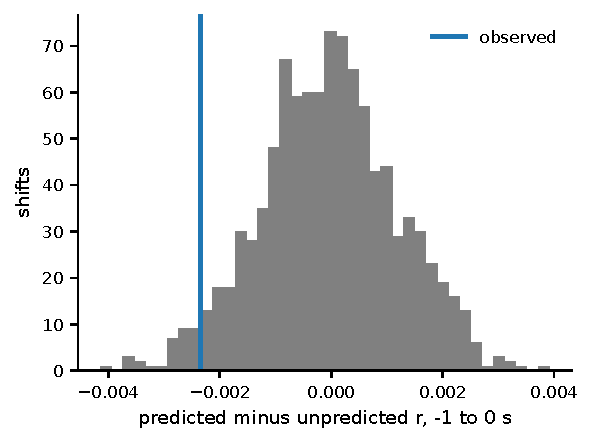
\includegraphics[width=0.55\textwidth]{sub-03-label-null.pdf}
\caption{Label-shift null for the predicted minus unpredicted difference in mean $r$ from $-1$ to 0\,s, averaged over the 185 significant electrodes (gray, 1,000 shifts). The blue line marks the observed difference.}
\label{fig:label}
\end{figure}

\paragraph{Encoding before word onset.}
All three models performed above their prediction-shift nulls from $-1$ to 0\,s, each at the p-value floor of 0.001 (Table~\ref{tab:window}). The previous-word model ($r = 0.0232$) performed above the current-word model ($r = 0.0214$) in this window, and did so in 117 of 185 electrodes. Across lags (Figure~\ref{fig:prev}, top), the previous-word and joint models peaked just before onset, at $-0.06$\,s ($r = 0.036$ and $0.041$), while the current-word model peaked at 0.25\,s ($r = 0.039$).

\begin{table}[htbp]
\centering
\caption{Mean encoding performance from $-1$ to 0\,s over the 185 significant electrodes, against the prediction-shift null (1,000 shifts).}
\label{tab:window}
\begin{tabular}{lrrr}
\toprule
Model & Observed $r$ & Null 95th percentile & p \\
\midrule
Current word  & 0.0214 & 0.0015 & 0.001 \\
Previous word & 0.0232 & 0.0015 & 0.001 \\
Joint         & 0.0255 & 0.0017 & 0.001 \\
\bottomrule
\end{tabular}
\end{table}

\paragraph{What the previous word explains.}
The unique variance of the current word from $-1$ to 0\,s was $U = 0.00040$, against a null 95th percentile of $0.000008$ ($p = 0.001$, the floor). This is 19\% of the joint model's mean $r^2$ in the window (0.0021), and 114 of 185 electrodes had positive unique variance. Within the window, unique variance was larger from $-0.5$ to 0\,s (0.00068) than from $-1$ to $-0.5$\,s (0.00022), and across lags it peaked after onset, at 0.34\,s (Figure~\ref{fig:prev}, bottom).

\begin{figure}[htbp]
\centering
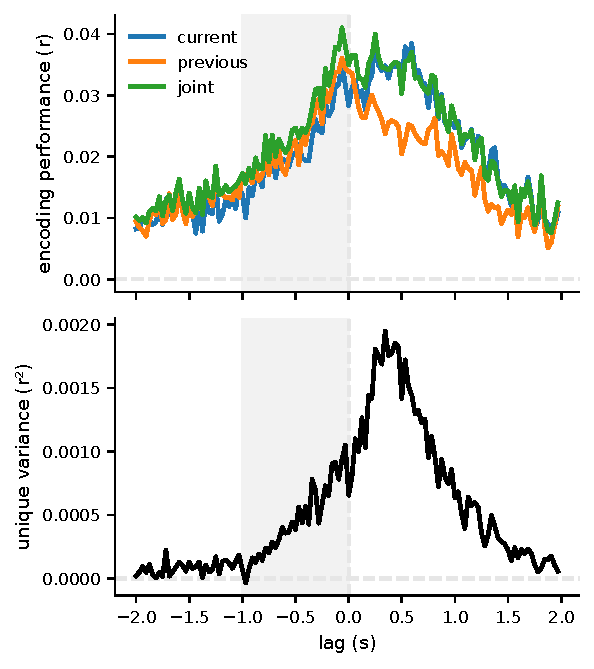
\includegraphics[width=0.55\textwidth]{sub-03-previous-word.pdf}
\caption{Top, encoding performance of the current-word, previous-word, and joint models, averaged over the 185 significant electrodes. Bottom, unique variance of the current word at each lag (Equation~\ref{eq:unique} applied lag by lag). The gray area marks $-1$ to 0\,s.}
\label{fig:prev}
\end{figure}

\section{Interpretation}

The group difference fell inside the label-shift null, so in sub-03 we found no evidence that GPT-2 XL's correct guesses change pre-onset encoding. The two-sided p-value of 0.057 is close to the conventional threshold, and the observed difference sits in the lower tail of the null, but it does not support the direction a prediction account expects, which would be higher encoding for predicted words.

Pre-onset encoding performance of the current-word model was above the prediction-shift null, so it is not explained by autocorrelation alone. Its size, however, is matched or exceeded by a model that sees only the previous word's embedding, consistent with part of the activity before a word's onset reflecting the response to the preceding word.

The current word still added unique variance beyond the previous word, meaning that it carries pre-onset information the previous word does not. This pattern is consistent with prediction, but three points limit that reading. First, a contextual embedding of the current word also carries information about words earlier than the immediately preceding one, so unique variance may reflect earlier context rather than a prediction of the upcoming word. Second, unique variance was concentrated in the half second before onset, where some of the post-onset response that the current word explains may spread across lags. Third, the prediction-shift null breaks the alignment of both models at once, so it tests unique variance against no alignment, not against a joint model whose current-word half carries no information. A stricter test would shift only the current-word features.

\section{Limitations}

\begin{enumerate}
\item All results come from one subject.
\item We ran on the CPU with the himalaya numpy backend. A 20-shift timing run put the full run at about 4.5\,h, which is what kept the null at 1,000 shifts. A GPU run with the torch backend may differ in the last digits.
\item The window from $-1$ to 0\,s was fixed in advance and not tuned. Other windows may give different results.
\item With 1,000 shifts, the smallest possible p-value is $1/1001 \approx 0.001$. The three window tests and the unique variance test all reached this floor, so their p-values are upper bounds and do not rank the four results against each other.
\end{enumerate}

\end{document}
